\documentclass{article} % For LaTeX2e
\usepackage{nips13submit_e,times}
\usepackage{hyperref}
\usepackage{url}
\usepackage{tikz}

\bibliographystyle{plain}
%\documentstyle[nips13submit_09,times,art10]{article} % For LaTeX 2.09


\title{Learning Human Activities and Object Functionalities through Conditional Random Fields}


\author{
Nakul Gopalan\\
Department of Computer Science\\
Brown University\\
Providence, RI 02912 \\
\texttt{ngopalan@cs.brown.edu} \\
\And
Jun Ki~Lee\\
Department of Computer Science\\
Brown University\\
Providence, RI 02912 \\
\texttt{jklee@cs.brown.edu} \\
}

% The \author macro works with any number of authors. There are two commands
% used to separate the names and addresses of multiple authors: \And and \AND.
%
% Using \And between authors leaves it to \LaTeX{} to determine where to break
% the lines. Using \AND forces a linebreak at that point. So, if \LaTeX{}
% puts 3 of 4 authors names on the first line, and the last on the second
% line, try using \AND instead of \And before the third author name.

\newcommand{\fix}{\marginpar{FIX}}
\newcommand{\new}{\marginpar{NEW}}

\nipsfinalcopy % Uncomment for camera-ready version

\begin{document}


\maketitle

\begin{abstract}
Recognizing a human activity is a skill that humans learn early in life. Activity recognition helps humans in predicting next steps of the activitiy in question and also in planning other activities with respect to the recognized activity. Our objective is to recognize human activities using machine learning, to predict next steps of an action, or provide help using robots or other interfaces, or help recognizing problems in the activity being performed. Specifically of interest to us are the human activities being performed on a table-top, where the human can be observed and helped by a robot. We plan to use a dataset from \cite{koppula2013detectingactivitiesrgbd} to learn a Graphical Model with temporal and spatial structure, which can then be used to predict the action being performed. As a baseline we have results of a bag of words classification of the $10$ activities, which yields a result of $67\%$.
\end{abstract}

\section{Introduction}
% why problem important, how object information and affoirdance/ functionality can help in recognizing an action

\section{Background}
% what has been tried previously why this work interests us as roboticists who work on the table top environment.....

\section{Dataset}
We explored data sets with activity labels and corresponding skeletal trajectories. Humans frequently perform activities using objects, especially in table-top scenarios. The dataset from \cite{koppula2013detectingactivitiesrgbd} was constructed keeping this relationship in mind. The raw data consists of the RGB-D frames from the scenes of humans performing activities and human skeletal poses from the OpenNI NITE tracker \cite{PrimeSense2010}. The skeletal poses are not precise and have confidence intervals. The labels on the data are related to both the objects present in the scene and the activities involved. Activity specific labels are framewise labels on subactivities	and the main activity being performed. The sub-activity labels are that of reaching, moving, pouring, eating, drinking, opening, placing, closing, scrubbing and null. The object specific labels consist of object location, object pose, object id and object affordance of the objects present in the scene. The object affordance lables are those of reachable, movable, pourable, pour to, containable, drinkable, openable, placeable, closable, scrubbable, scrubber and stationary. The dataset also has precomputed features that have relationship between objects and skeletal poses across frames. 
For the experiments performed in this proposal we use only skeleton pose data, but for our next set of results we would use the pairwise relationship between objects and the skeleton data, and also the temporal features of data available.

%The data consisits of skeletal poses of human subjects performing activities, but along with this the dataset also has lables, positions and poses for all objects present in the scene. The activities present in the dataset are: cleaning, stacking objects, unstacking objects, eating, making cereal, taking medicine, microwaving food, arranging objects, taking food and picking objects. The activities themselves have been broken down into subactivities like placing, reaching, grabbing, which are labelled framewise. 

\section{Methods}
The data from \cite{koppula2013detectingactivitiesrgbd} has a lot of structure, temporal and within the frame relationships between objects and skeleton positions. The authors from \cite{koppula2013detectingactivitiesrgbd} modelled this structure using a pairwise graphical model as shown in Fig.~\ref{fig:model}.
As a baseline for our experiments we create a try to classify skeletal trajectories using a Bag of Words model \cite{Sivic03} with skeletal poses as features.

\begin{figure}[t]
\centering

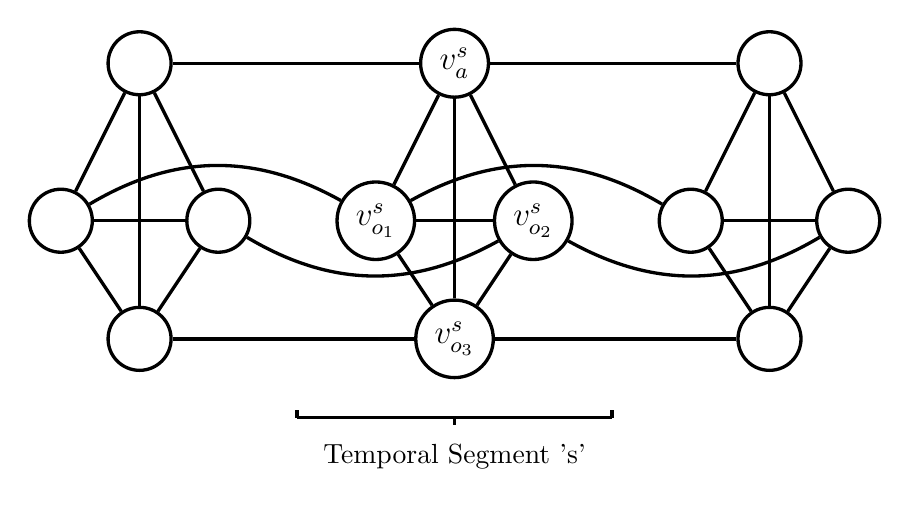
\begin{tikzpicture}[-,auto,very thick,main node/.style={circle,draw, minimum size=0.8cm, font=\large}]
  \node[main node] (a1) at (1, 3.5) {};
  \node[main node] (a2) at (1, 0) {};
  \node[main node] (a3) at (0, 1.5) {};
  \node[main node] (a4) at (2, 1.5) {};
  \node[main node] (b1) at (5, 3.5) {$v_a^s$};
  \node[main node] (b2) at (5, 0) {$v_{o_3}^s$};
  \node[main node] (b3) at (4, 1.5) {$v_{o_1}^s$};
  \node[main node] (b4) at (6, 1.5) {$v_{o_2}^s$};
  \node[main node] (c1) at (9, 3.5) {};
  \node[main node] (c2) at (9, 0) {};
  \node[main node] (c3) at (8, 1.5) {};
  \node[main node] (c4) at (10, 1.5) {};
  \path
	(a1) edge (a2)
    (a1) edge (a3)
    (a1) edge (a4)
    (a2) edge (a3)
    (a2) edge (a4)
    (a3) edge (a4)
	(b1) edge (b2)
    (b1) edge (b3)
    (b1) edge (b4)
    (b2) edge (b3)
    (b2) edge (b4)
    (b3) edge (b4)
	(c1) edge (c2)
    (c1) edge (c3)
    (c1) edge (c4)
    (c2) edge (c3)
    (c2) edge (c4)
    (c3) edge (c4)
    (a1) edge (b1)
    (b1) edge (c1)
    (a2) edge (b2)
    (b2) edge (c2)
    (a3) edge [bend left] (b3)
    (b3) edge [bend left] (c3)
    (a4) edge [bend right] (b4)
    (b4) edge [bend right] (c4);
  \draw[very thick] (3, -1)--(7, -1);
  \draw[very thick] (3, -1)--(3, -0.9);
  \draw[very thick] (7, -1)--(7, -0.9);
  \draw[very thick] (5, -1)--(5, -1.1);
  \node at (5, -1.5) {Temporal Segment 's'};
\end{tikzpicture}
\caption{ MRF }
\label{fig:model}

\end{figure}




\bibliography{ref}


\end{document}
